\chapter{The Experiment}

\begin{figure}[h]
\centering
\begin{subfigure}[b]{0.8\textwidth}
                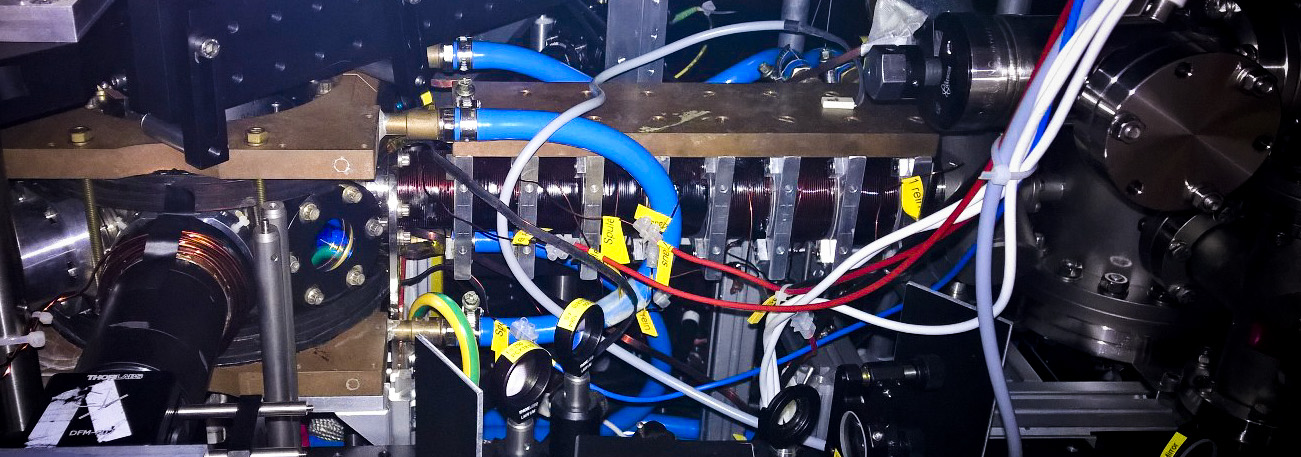
\includegraphics[width=\textwidth]{experiment}
\end{subfigure}
\caption{Photograph of the core-part of the experiment. On the left the octagon-shaped vacuum chamber is visible, with viewports and lenses, focussing beams for the optical dipole trap and the \textsc{mot}. On the right one can see the oven and the Zeeman-slower connecting both parts.}
\label{experiment}
\end{figure}
The key feature of the experiment is the possibility to prepare few atoms in a microscopic dipole trap with high control over their number. A precise description of the experiment is found in \cite{friedhelm}. A briefer summary of this is given in this paragraph.

The experiments are carried out in the so called microtrap, that for the lowest occupied levels can be approximated by a one-dimensional harmonic oscillator. To fill this potential down to the ground state a big reservoid of cold atoms has to be prepared before activating this main stage of the experiment.

After vaporizing Lithium in an oven, the first component of the experiment is the Zeeman slower. When leaving the oven, the atoms are very hot and propagate at velocities, that are too large to trap them in the \textsc{mot} or dipole trap. The Zeeman-slower reduces this speed using radiation pressure while adapting for the the different doppler shifts, exploiting the Zeeman-effect. The slower is essentially a large tube behind the oven shutter surroundet by coils, that provide a different magnetic field value at every point of the apperatus. A strong laserbeam is pointing along the slower. When the beam is in resonance with an atomic transition, the photons get absorbed and the atoms are pushed in the direction of the laser. Because the spontanious emission is directed in random directions, this leads to slowing of the cloud. The atoms however, due to the Doppler-effect see the light blue detuned when flying at high velocities. If the frequency of the laser-beam is adapted to match the resonance frequency for the respective speed, the atoms will be slowed down, but therefore will no longer absorb photons of the same frequency. Therefore different magnetic fields shifts the atomic levels to match the frequncy of the laser everywhere along the legth of the tube and achieve enough cooling to trap the atoms in the \textsc{mot}. 

It consists of six counterpropagating near-resonsant laser-beams. The usage of many retroreflected beams in different directions make it possible to not only force the atoms in a certain direction like in the Zeeman-slower, but to affect all of them with a high absolute speed value and push in the opposite way, in this manner reducing the overall average-speed and therefore cooling the gas. However, because the force of the laserbeams alone is only velocity-dependent, slow particles would exit the center of the crossed beams over time. That is why in a magneto-optical trap a magnetic quadrupole-field is applied, that has zero strength in the middle and will increase when moving further away from the center. The Zeeman-effect shifts the level-distace for the outmoving atoms towards the frequency of the laser, which will then apply a force, dependent on the spatial position, enabeling not only cooling but trapping and compression of the gas-sample. The natural linewith of the used transition limits the cooling of the \textsc{mot} to a temperature of around 140 \mu K. The system used in this experiment can store around 10⁸ atoms. 

The temperature however has to be reduced much further to match the requirements of the experiment later on. The next step on this ladder is the crossed dipole trap. \begin{figure}[h]
\centering
\begin{subfigure}[b]{0.8\textwidth}
                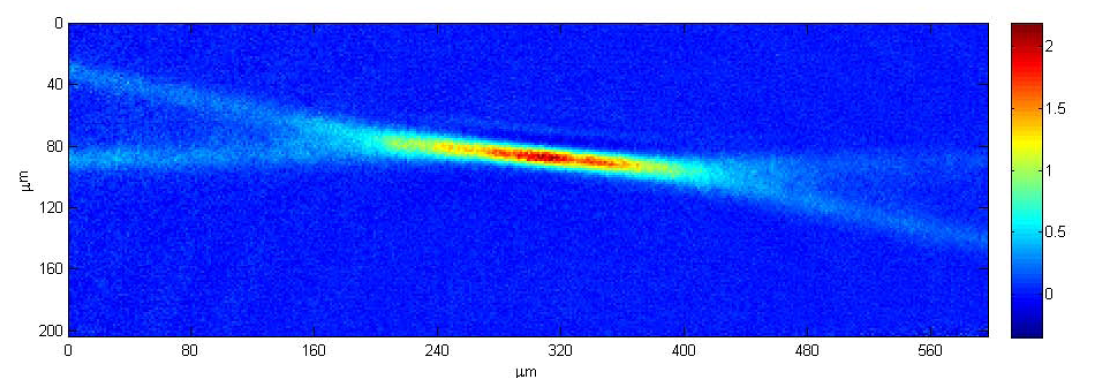
\includegraphics[width=\textwidth]{dipolefoto}
\end{subfigure}
\caption{Absorbtion image of the crossed dipole trap \cite{lompe}.}
\label{experiment}
\end{figure}
It uses the laserbeam of a 200 W Ytterbium fiber-laser (\textsc{ipg ylr-200-lp}) that is far red-detuned from the atomic transitions at 1070 nm. The beams focus lies within the \textsc{mot}, with a waist of approximately 40 \mu m \cite{lompe}. After leaving the vacuum chamber, a mirror system guides it back in at a different angle, forming the crossed trap shape. To trap the most atoms possible the laser is ramped up to full power, leading to a trap depth of over 3 mK. To further cool the sample the power is slowly ramped down, so the hottest atoms escape the potential and the rest of the cloud thermalises at a lower temperature (evaporative cooling). A small, tightly focussed infrared laser-beam at 1064 nm, that intersects the crossed dipole-trap then formes the microtrap (\textsc{mephisto S} from Innolight). The small dimensions of the trap result in high spacing between the allowed harmonic vibrational levels. To control the atom number in the microtrap, a magnetic field gradient tilts the dipole-potential. That leads to the escape of all atoms above a certain level and using this technique one can control the number of atoms between 0 and 10 atoms with high preperation fiddelity. To see the atoms, the microtrap is shut down and the remaining atoms are again trapped in a smaller \textsc{mot}. The resulting flourescence is caught by an objective and projected at the sensor of a \textsc{ccd}-camera. 
\begin{figure}[h]
\centering
\begin{subfigure}[b]{0.8\textwidth}
                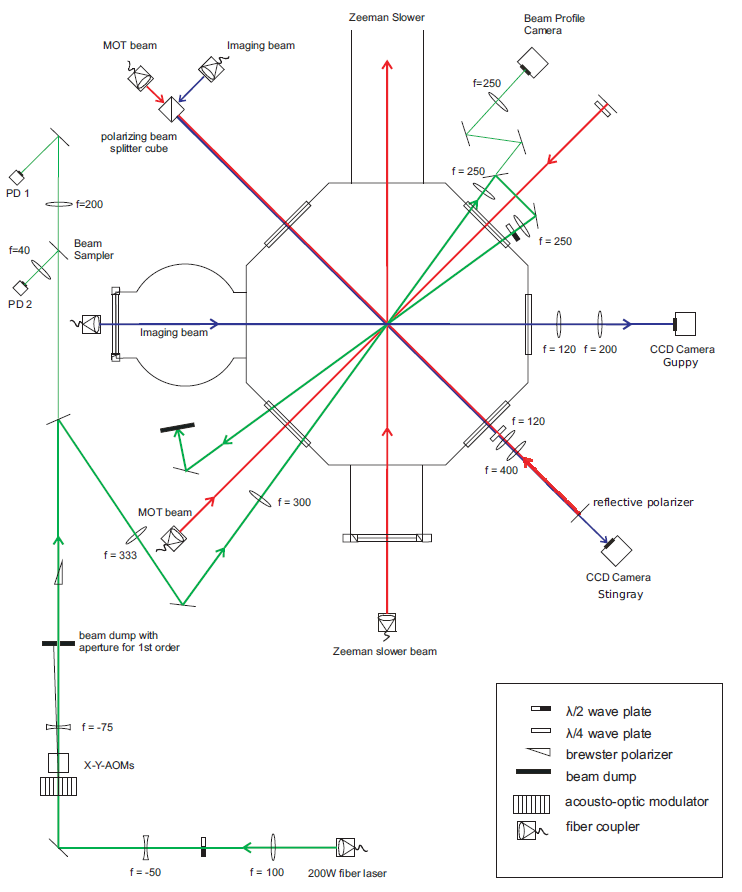
\includegraphics[width=\textwidth]{scheme}
\end{subfigure}
\caption{Scheme of the laser set-up around the vacuum chamber \cite{lompe}. }
\label{scheme}
\end{figure}

